\chapter{Design der Software}
\label{sec:design}

\section{UML Diagramm des Modells}
\label{sec:design:UML}
\begin{figure}[htb]
	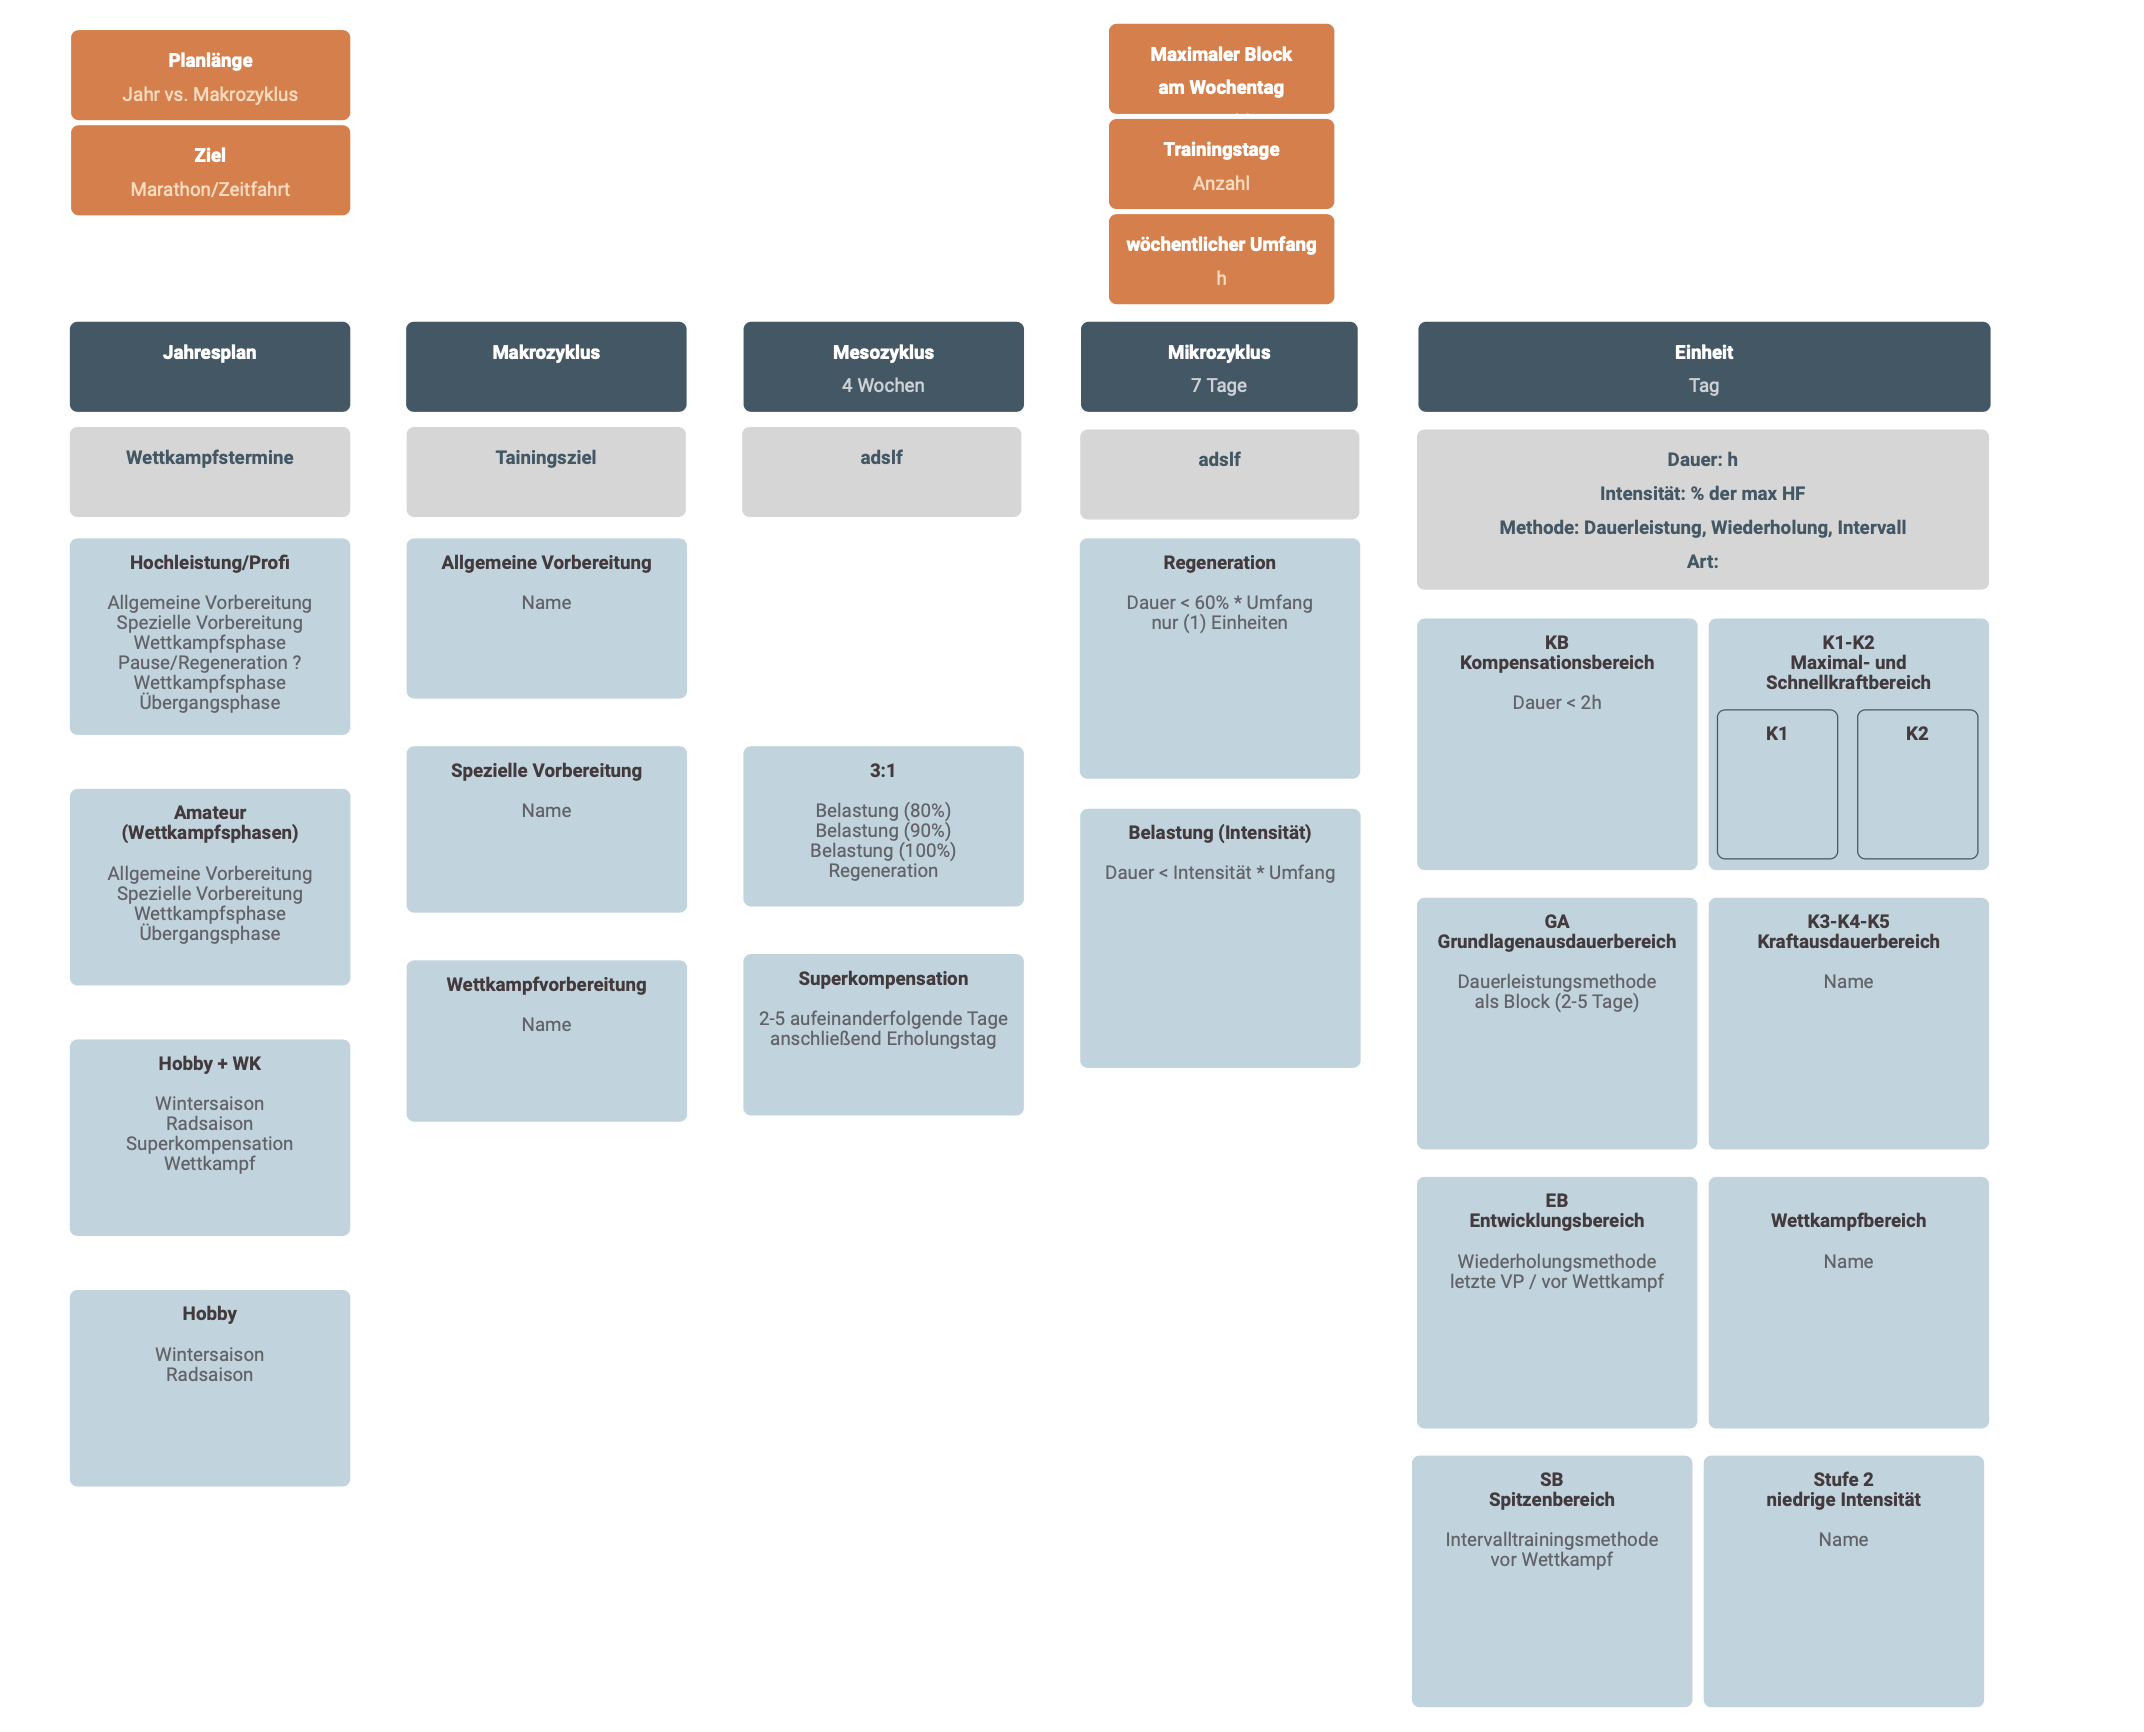
\includegraphics[width=\textwidth]{gfx/uml.png}
	\caption{UML Diagramm}
	\label{fig:system:example1}
\end{figure}
Objektorientiert nach hierarchischer Struktur der Zyklen.
Die Optimierung findet auf Ebene der Mesozyklen statt, sodass auch eine Parallelisierung der ein
\subsection{Trainingseinheit}
    Siehe Kapitel \ref{sec:modellierung}
\subsection{Trainingsplan}
    Als Liste von Trainingseinheiten oder Zyklische Struktur übernehmen
 
\section{Template Design Pattern}
\label{sec:design:template}
Template Method um verschiedene Wettkampfsarten umzusetzen

